\documentclass{article}
\usepackage{blindtext}
\usepackage{listings}
\usepackage[english]{babel}
\usepackage{hyperref}
\usepackage{comment}
\usepackage[backend=biber, sorting=none]{biblatex}
\nocite{*}
\usepackage{xcolor}
\usepackage{subcaption}
\usepackage{graphicx}
\hypersetup{
    colorlinks,
    linkcolor={red!50!black},
    citecolor={blue!50!black},
    urlcolor={blue!80!black}
}
\addbibresource{sample.bib}

\usepackage{svg}
\usepackage{fancyhdr}
\usepackage{lipsum}

\pagestyle{fancy}
\headheight=14pt

\fancyhf{}
\font\myfont=cmr12 at 24pt
\lhead{\small{Faiella Ciro, Giannino Pio Roberto, Scovotto Luigi and Tortora Francesco}}
\rhead{\small{\thepage}}

\title{\textbf{\myfont Autonomous Vehicle Driving: Group 8}}
\author{\small{Faiella Ciro, Giannino Pio Roberto, Scovotto Luigi and Tortora Francesco}}
\date{\small{\{\href{mailto:c.faiella8@studenti.unisa.it}{c.faiella8}, \href{mailto:p.giannino@studenti.unisa.it}{p.giannino}, \href{mailto:l.scovotto1@studenti.unisa.it}{l.scovotto1}, \href{mailto:f.tortora21@studenti.unisa.it}{f.tortora21}\}@studenti.unisa.it}}

\makeindex

\begin{document}
\maketitle
\centerline{\small{Jun, 2023}}
\centerline{Department of Computer Engineering, Electrical Engineering and Applied}
\centerline{Mathematics (DIEM), University of Salerno, Fisciano, Italy}


\section{Introduction}
The project focuses on the creation of an autonomous driving system to be included in the CARLA simulator 
environment. Unlike the task performed in the real world, in this case there is full knowledge of the world 
in which the vehicle is located, nevertheless the system has to face several challenges in order to avoid 
errors. 

\section{Development environment}
\subsection{Hardware}
We conducted the software testing on a Dell machine equipped with an NVIDIA Quadro P2000 graphics card, boasting 4GB of dedicated memory. 
The system was powered by an Intel 8th generation i9 processor, delivering exceptional processing power. Furthermore, it was equipped with a 
substantial 16GB of RAM, ensuring smooth and efficient operation throughout the testing phase.
In order to optimize performance and enhance the execution speed, we opted to remove all unnecessary sensors from the machine, 
as they were not utilized during the testing process. Leveraging our comprehensive global knowledge of the surrounding environment, 
we were able to confidently eliminate these redundant components. 
As a result, the execution speed experienced a notable improvement, exhibiting an impressive 30\% increase compared to the performance of
the machine provided to us by the department.

\subsection{CARLA Simulator}
???

\section{Task}
The CARLA AD Leaderboard challenges AD agents to drive through a series of predefined routes. For each route, 
agents are initialized at a starting point and directed to a destination point with a route description. 
Routes are defined in a variety of situations, including urban areas, residential neighborhoods and rural environments. 
The classification evaluates AD agents in different weather conditions, including daytime scenes, sunset, rain, fog and night.

\section{Operational Design Domain}
First of all, considering the fact that the data used by the ego-vehicle are directly provided by CARLA simulator and they are not took by any kind of sensor, we have 
that the our ODD has reached the following operational domains:
\begin{itemize}
    \item the vehicle is able to maintain the selected speed, thanks the longitudinal control;
    \item the vehicle is able to maintain the correct position between the lanes of a road thanks to the lateral control;
    \item the vehicle is able to manage its speed in according to the variable traffic conditions;
    \item the vehicle is able to avoid collisions with the car ahead and adapts its speed in order to follow that one;
    \item the vehicle is capable of overtaking when possible and when necessary;
    \item the vehicle is capable to makes an emergency stop in critical situations;
    \item the vehicle is able to operate in sunny, foggy, raining and poor lighting environments;
    \item the vehicle can operate in urban and non-urban contexts;
    \item the vehicle is capable of handling junctions;
    \item the vehicle is able to avoid collisions with obstacles that can be find through the path (e.g. road cones, traffic sign, construction obstacle, etc.);
    \item the vehicle is able to correctly pass the traffic light.
\end{itemize}

\subsection{Traffic Scenario}
Agents will experience multiple instances of 10 traffic scenarios selected from the NHTSA pre-crash typology \cite{NHTSA}. 

\subsubsection{Control loss}
The ego-vehicle loses control due to bad conditions on the road and it must recover, coming back to its original lane.
\begin{figure}[h]
    \centering
    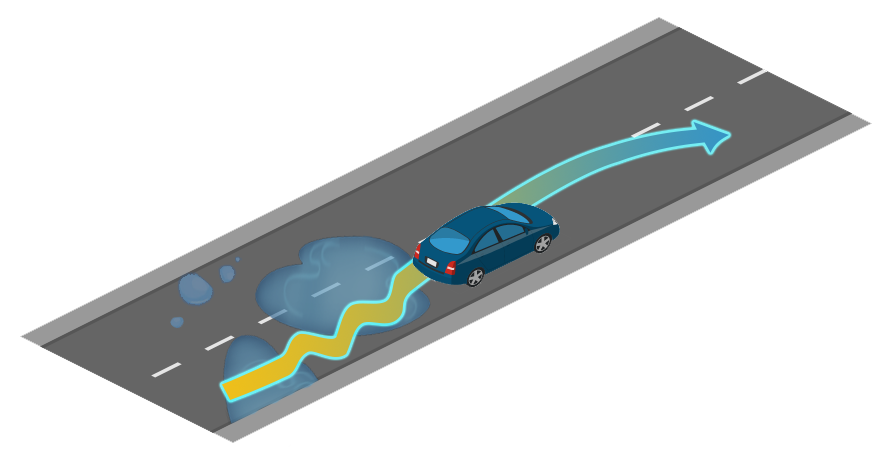
\includegraphics[width=0.5\textwidth]{img/TR01.png}
    \caption{Control loss without previous action} \label{Scenario_controlLoss}
\end{figure}

\subsubsection{Traffic negotiation}
\textbf{Unprotected left turn at intersection with oncoming traffic}
The ego-vehicle is performing an unprotected left turn at an intersection, yielding to oncoming traffic. This scenario occurs at both signalized and non-signalized junctions.
\begin{figure}[h]
    \centering
    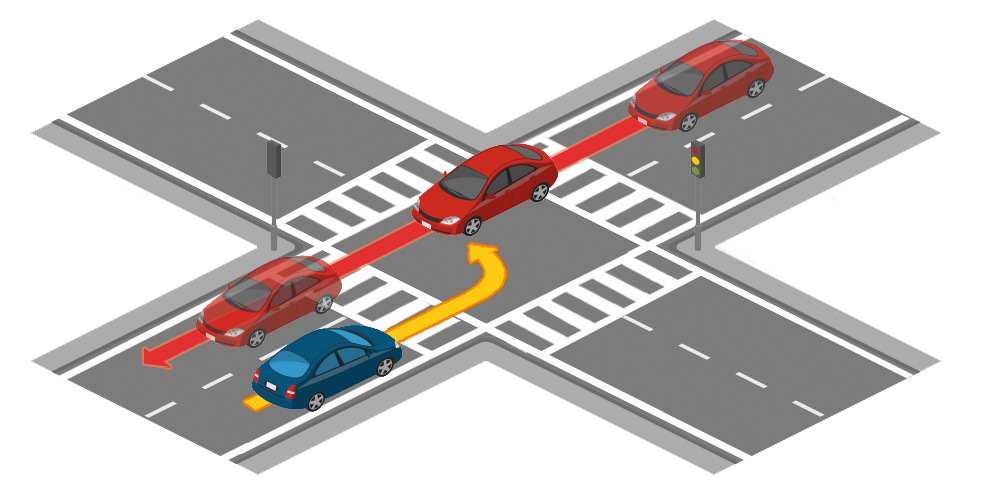
\includegraphics[width=0.5\textwidth]{img/TR08.png}
    \caption{Right turn at an intersection with crossing traffic} \label{Scenario_trafficNegtiation}
\end{figure}

\textbf{Right turn at an intersection with crossing traffic} 
The ego-vehicle is performing a right or left turn at an intersection, yielding to crossing traffic. This scenario occurs at both signalized and non-signalized junctions.
\begin{figure}[h]
    \centering
    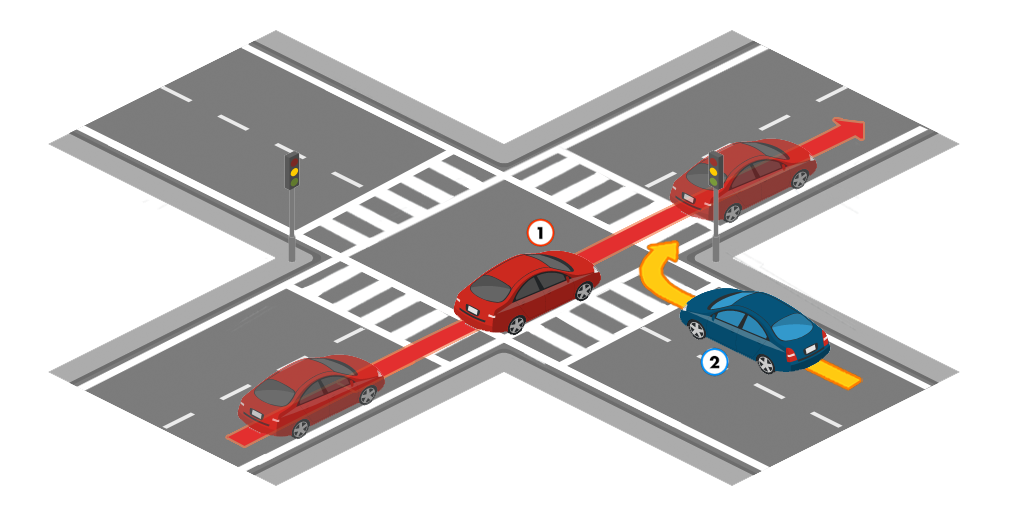
\includegraphics[width=0.5\textwidth]{img/TR09.png}
    \caption{Right turn at an intersection with crossing traffic} \label{Scenario_trafficNegtiation}
\end{figure}

\textbf{Crossing negotiation at an unsignalized intersection} 
The ego-vehicle needs to negotiate with other vehicles to cross an unsignalized intersection. In this situation it is assumed that the first to enter 
the intersection has priority.
\begin{figure}[h]
    \centering
    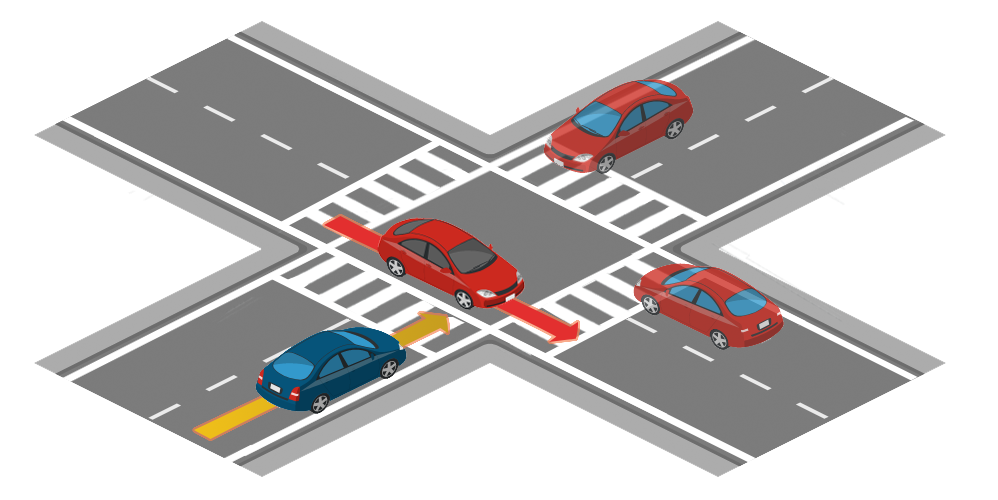
\includegraphics[width=0.5\textwidth]{img/TR10.png}
    \caption{Crossing negotiation at an unsignalized intersection} \label{Scenario_crossingNegotiation}
\end{figure}

\subsubsection{Obstacle avoidance}
\textbf{Obstacle in lane} 
The ego-vehicle encounters an obstacle blocking the lane and must perform a lane change into traffic moving in the opposite direction to avoid it. 
The obstacle may be a construction site, an accident or a parked vehicle.
\begin{figure}[h]
    \centering
    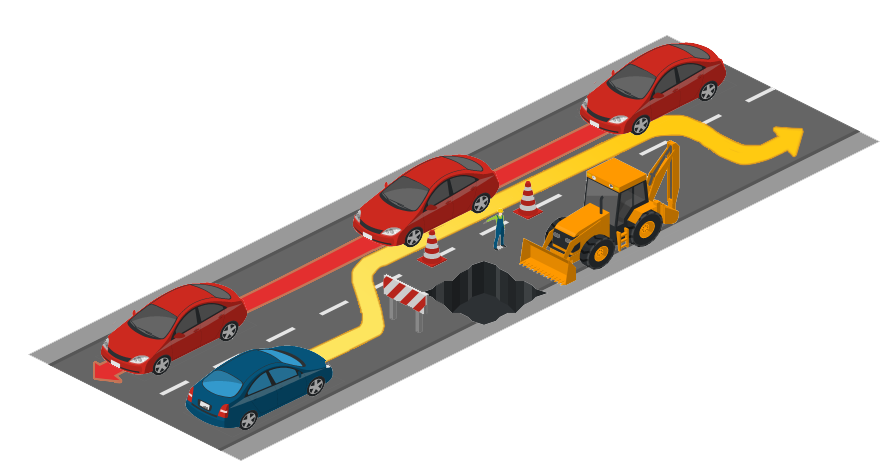
\includegraphics[width=0.5\textwidth]{img/TR14a.png}
    \caption{Obstacle in lane} \label{Scenario_obstacle}
\end{figure}

\textbf{Slow moving hazard at lane edge} 
The ego-vehicle encounters a slow moving hazard blocking part of the lane. The ego-vehicle must brake or maneuver to avoid it next to a lane of traffic 
moving in the opposite direction.
\begin{figure}[h]
    \centering
    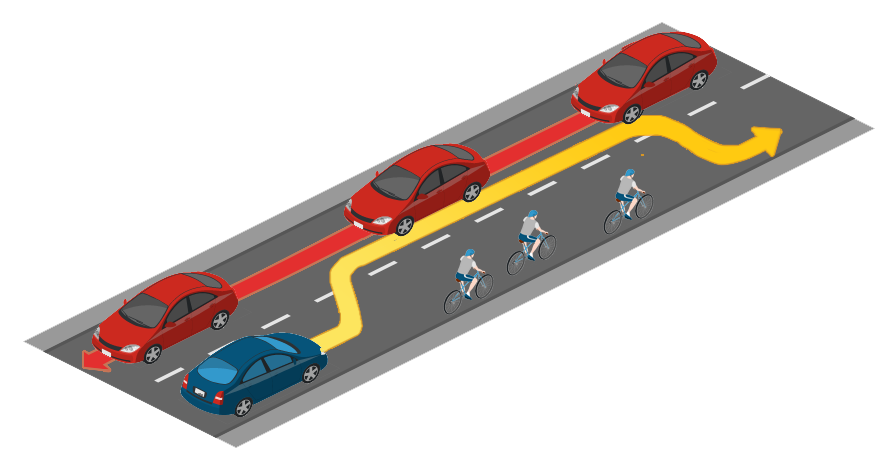
\includegraphics[width=0.5\textwidth]{img/TR16a.png}
    \caption{Slow moving hazard at lane edge} \label{Scenario_slowMove}
\end{figure}

\textbf{Vehicle invading lane on bend} 
The ego-vehicle encounters an oncoming vehicles invading its lane on a bend due to an obstacle. It must brake or maneuver to the side of the road 
to navigate past the oncoming traffic.
\begin{figure}[h]
    \centering
    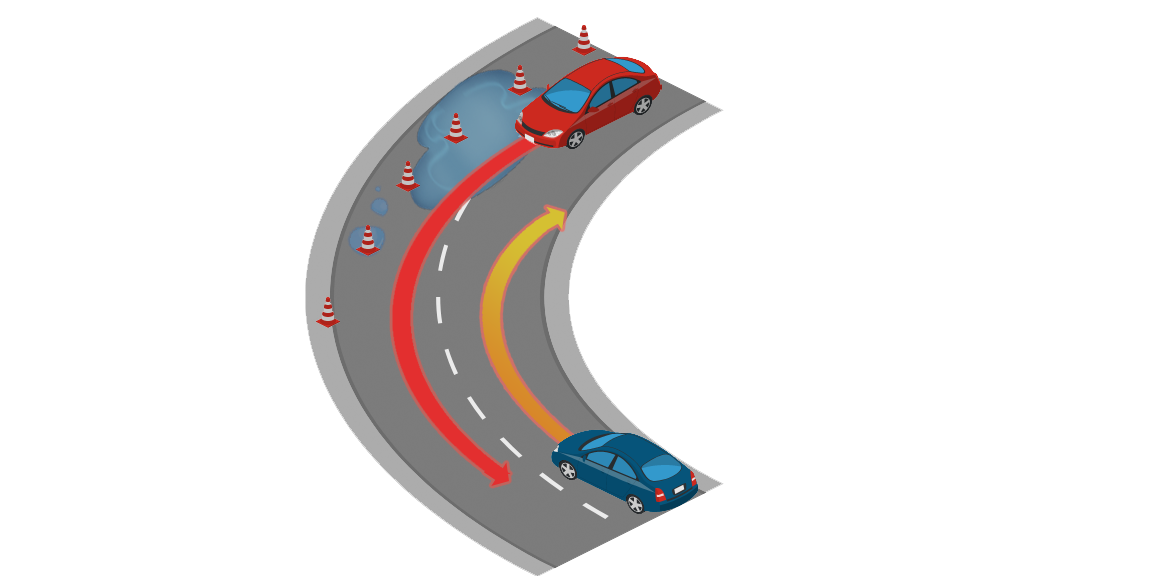
\includegraphics[width=0.5\textwidth]{img/TR22.png}
    \caption{Vehicle invading lane on bend} \label{Scenario_vehicleInvading}
\end{figure}

\subsubsection{Braking and lane changing}
\textbf{Longitudinal control after leading vehicle’s brake} 
The leading vehicle decelerates suddenly due to an obstacle and the ego-vehicle must perform an emergency brake or an avoidance maneuver.
\begin{figure}[h]
    \centering
    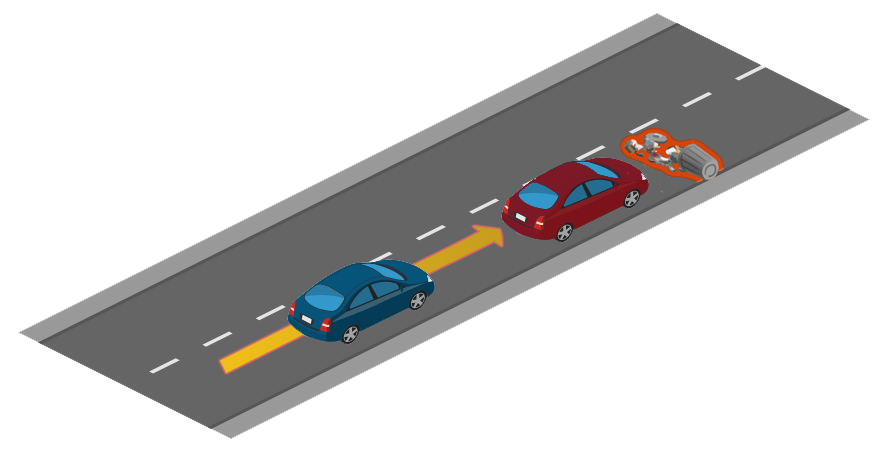
\includegraphics[width=0.5\textwidth]{img/TR02.png}
    \caption{Longitudinal control after leading vehicle’s brake} \label{Scenario_longgitudinalControl}
\end{figure}

\textbf{Obstacle avoidance without prior action} 
The ego-vehicle encounters an obstacle / unexpected entity on the road and must perform an emergency brake or an avoidance maneuver.
\begin{figure}[h]
    \centering
    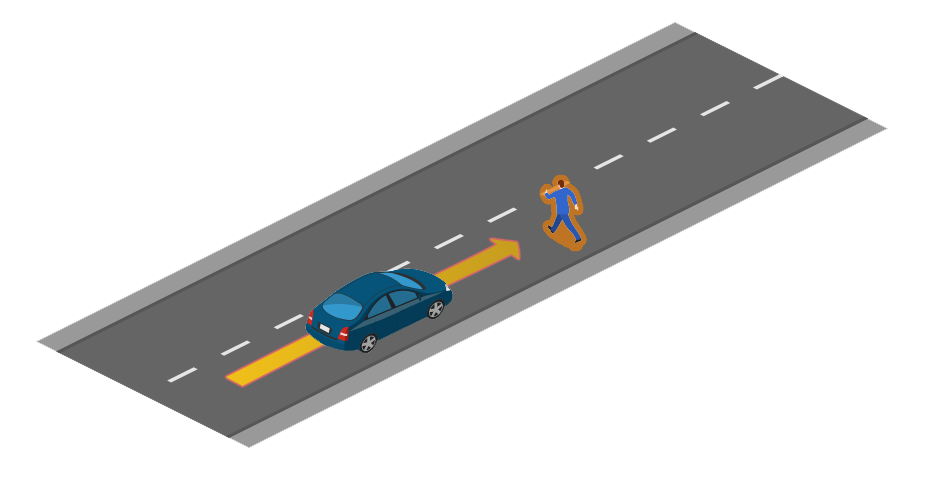
\includegraphics[width=0.5\textwidth]{img/TR03.png}
    \caption{Obstacle avoidance without prior action} \label{Scenario_obsAvoidanceWithout}
\end{figure}

\textbf{Pedestrian emerging from behind parked vehicle} 
The ego-vehicle encounters an pedestrian emerging from behind a parked vehicle and advancing into the lane. The ego-vehicle must brake or maneuver to avoid it.
\begin{figure}[h]
    \centering
    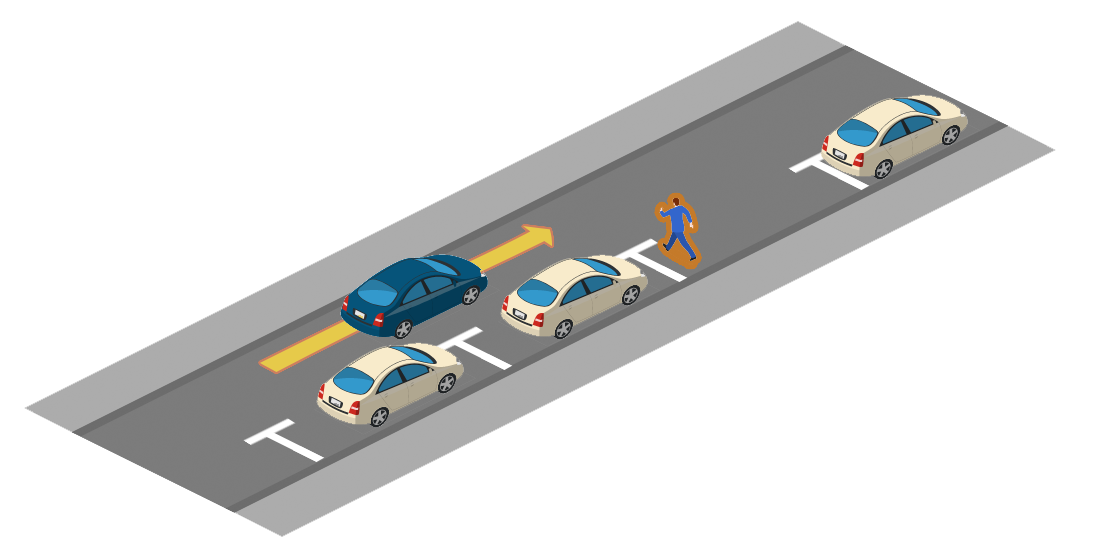
\includegraphics[width=0.5\textwidth]{img/TR17.png}
    \caption{Pedestrian emerging from behind parked vehicle} \label{Scenario_pedestrianEmerging}
\end{figure}

\textbf{Obstacle avoidance with prior action - pedestrian or bicycle} 
While performing a maneuver, the ego-vehicle encounters an obstacle in the road, either a pedestrian or a bicycle, and must perform an emergency brake 
or an avoidance maneuver.
\begin{figure}[h]
    \centering
    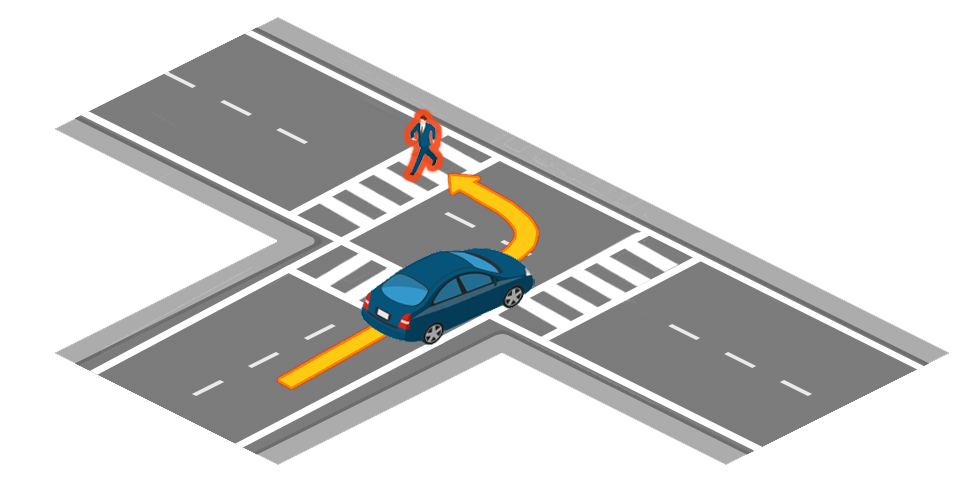
\includegraphics[width=0.5\textwidth]{img/TR04.png}
    \caption{Obstacle avoidance with prior action - pedestrian or bicycle} \label{Scenario_obsAvoidanceWithPedBic}
\end{figure}

\textbf{Obstacle avoidance with prior action - vehicle} 
While performing a maneuver, the ego-vehicle encounters a stopped vehicle in the road and must perform an emergency brake or an avoidance maneuver.
\begin{figure}[h]
    \centering
    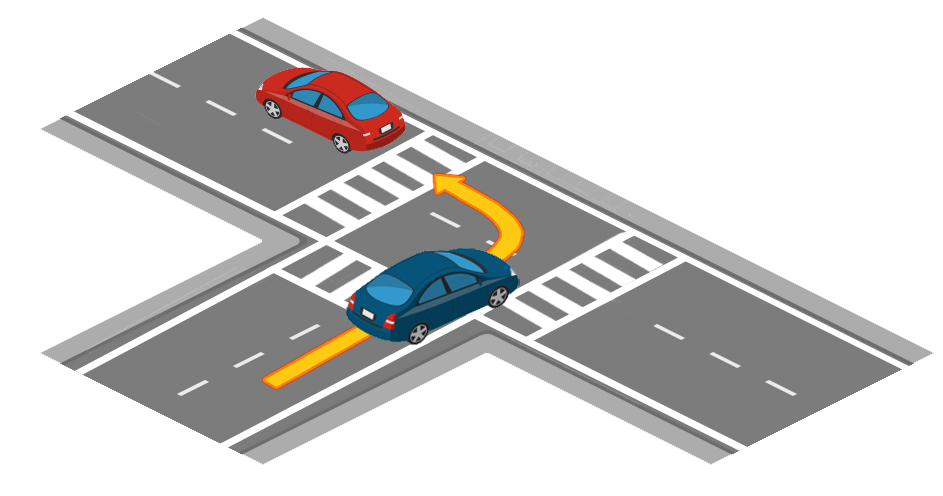
\includegraphics[width=0.5\textwidth]{img/TR19a.png}
    \caption{Obstacle avoidance with prior action - vehicle} \label{Scenario_obsAvoidanceWithoutVehicle}
\end{figure}

\section{Vehicle configuration}

\subsection{Control system}

\section{Evaluation and metrics}
The driving proficiency of an agent can be characterized by multiple metrics. For the assigned leaderboard, we have a number of metrics that help 
to understand different aspects of driving. Although all routes have the same type of metrics, the respective values are calculated separately. 
The specific metrics are as follows:
\begin{itemize}
  \item \textbf{Driving score}: Product between the route completion and the infraction penalty, $R_i P_i$. Main metric of the leaderboard, 
  serving as the product between the route completion and the infractions penalty. Here Ri is the percentage of completion of the \textit{i-th} route, and \textit{Pi}, 
  the infraction penalty of the \textit{i-th} route.
  \item \textbf{Route completion}: Percentage of the route completed by the agent. The route completion is calculated as the percentage of the route
  \item \textbf{Infraction penalty}: Productory of the infractions committed, $\prod_{j}^{ped., ..., stop} (a_{\small{i}}^{\small{j}})^{\small{\#infractions}_j}$. — The leaderboard 
  tracks several types of infractions and this metric aggregates all of these infractions triggered by an agent as a geometric series. Agents start with an ideal 1.0 
  base score, which is reduced each type an infraction is committed.
\end{itemize}
When all routes have been completed, a global metric for each of the previous three types is also generated, being the arithmetic mean of all the individual routes combined. 
The global driving score is the main metric on which you will be classified with respect to other participants.

\subsection{Infractions and shutdown events}
The CARLA leaderboard offers individual metrics for a series of infractions. Each of these has a penalty coefficient that will be applied everytime it happens. 
Ordered by severity, the infractions are the following.
\begin{itemize}
    \item \textbf{Collisions with pedestrians} - $a_{\small{i}}^{\small{ped.}} = 0.60$
    \item \textbf{Collisions with vehicles} - $a_{\small{i}}^{\small{veh.}} = 0.50$
    \item \textbf{Collisions with static elements} - $a_{\small{i}}^{\small{statEl.}} = 0.65$
    \item \textbf{Running a red light } - $a_{\small{i}}^{\small{light.}} = 0.70$
    \item \textbf{Stop sign} - $a_{\small{i}}^{\small{stop.}} = 0.80$
    \item \textbf{Scenario timeout} - $a_{\small{i}}^{\small{time.}} = 0.70$. Some scenarios feature behaviors that can block the ego-vehicle indefinitely. 
            These scenarios will have a timeout of 4 minutes after which the ego-vehicle will be released to continue the route. However, a penalty is applied when 
            the time limit is breached.
    \item \textbf{Failure to maintain minimum speed} - $a_{\small{i}}^{\small{speed.}} = 0.70$. The agent is expected to maintain a minimum speed in keeping with nearby traffic.
            The agent’s speed will be compared with the speed of nearby vehicles. Failure to maintain a suitable speed will result in a penalty.
    \item \textbf{Failure to yield to emergency vehicle} - $a_{\small{i}}^{\small{yield.}} = 0.70$. The agent should yield to emergency vehicles coming from behind. Failure to allow the emergency vehicle to pass will incur a penalty.
    \item \textbf{Off-road driving} - If an agent drives off-road, that percentage of the route will not be considered towards the computation of the route completion score.
\end{itemize}

Additionally, some events will interrupt the simulation, preventing the agent to continue. In these cases, the route which is being simulated will be shut down, and the 
leaderboard will move onto the next one, triggering it normally.
\begin{itemize}
    \item \textbf{Route deviation} — If an agent deviates more than 30 meters from the assigned route.
    \item \textbf{Agent blocked} — If an agent doesn’t take any actions for 180 simulation seconds.
    \item \textbf{Simulation timeout} — If no client-server communication can be established in 60 seconds.
    \item \textbf{Route timeout} — If the simulation of a route takes too long to finish.
\end{itemize}

\section{Project development and phases }
The main problems were determined in order to define the problem domain (more on this in section x.xx). 
From this, we moved on to the development of solutions, with the highest priority problems being developed first.
\subsection{Controllers}
settaggio dei Controllori

One of the first tasks was the configuration of the controller, in order to determine a driving behavior 
that would seem as natural as possible. 
\subsubsection{PID Controller}
The PID controller was configured on the basis of several initial attempts. They led to the following values:
$$"longitudinal\_control\_dict" : {"K_P": 0.888 , "K_I": 0.0768, "K_D": 0.05, "dt": 0.05}$$
\subsubsection{Stanley Controller}
controllore di stanley

COSA DIRE?????

$$"lateral\_control\_dict" : {"K_V": 4, "K_S": 1, "dt": 0.05}$$

\subsection{Obstacle avoidance}
gesitone dell overtake

The development of the overtaking manoeuvre was one of the most challenging tasks due to its importance 
within such a system; its difficulty was such that it required constant development of this feature during 
the course of the entire project. The solution found is optimal in the context in which the vehicle moves, 
with no errors in the management of the various events.
The steps to manage overtake are the following:
\begin{enumerate}
    \item 
    \item 
    \item 
\end{enumerate}


\subsection{Stop sign}
Another phase concerned the management of stops; after trying countless solutions, we arrived at a solution that 
uses the static textit{*stop}. What we do, is to take all the stops in the scenario and evaluate whether they 
affect the ego-vehicle. 
Management begins by taking all stop signals and putting them into a listings, then the system follows these steps:
\begin{enumerate}
    \item for each stop sign, evaluate the distance between the stop sign and the ego-vehicle and discarding all distant stops;
    \item sort the remaining stops by the minimum distance;
    \item check all vehicles coming from the right and left.
\end{enumerate}
Now we have all the informations that we needed, so the ego-vehicle follows this behavior:
\begin{itemize}
    \item if there is no vehicle in the left and right lane, the stop sign is not affecting the vehicle;
    \item if there is a vehicle in the left lane, check if it is still affecting the vehicle;
    \item if there is a vehicle in the right lane, check if it is still affecting the vehicle;
    \item otherwise, the ego-vehicle can go.
\end{itemize}
 

\subsection{Invading lane}
gestione dell'invasione della corsia
There was also a phase where we handled lane invasion, since there are lane restrictions within the routes. 
The solution to this problem is the following:
\begin{enumerate}
    \item 
    \item 
    \item 
\end{enumerate}

\subsection{Pedestrian}
The management of vehicle behaviour in the presence of pedestrians was partly carried out, 
although there was not enough time for full development of the solution (more on this in section x.xx). 


\subsection{Traffic negotiation}
gestione degli incroci




\section*{Road Event Management}
In this section we will explain how we handled certain situations that occurred in the routes, 
in order to show the level of attention achieved by our system. The following subsections are 
correlated with demonstration videos to prove the effective functioning of the system.
\subsection*{Overtake}
\subsection*{Junction}
\subsection*{Lane invasion}







\section{Analisi qualitativa dei risultati}
scrivere dove siamo arrivati mostrando i video (minuti) e fare il confronto tra prima e dopo l'ottimizzazione
\subsection{Control loss}
testo con video

\subsection{Traffic negotiation}
\subsubsection{Right or left turn at an intersection with crossing traffic}
testo con video
\subsubsection{Crossing negotiation at an unsignalized intersection}
testo con video

\subsection{Obstacle avoidance}
\subsubsection{Obstacle in lane}
testo con video
\subsubsection{Slow moving hazard at lane edge}
testo con video 
\subsubsection{Vehicle invading lane on bend}
testo con video

\subsection{Braking and lane changing}
\subsubsection{Longitudinal control after leading vehicle’s brake}
testo con video
\subsubsection{Obstacle avoidance without prior action}
testo con video
\subsubsection{Pedestrian emerging from behind parked vehicle}
testo con video
\subsubsection{Obstacle avoidance with prior action - pedestrian or bicycle}
testo con video
\subsubsection{Obstacle avoidance with prior action - vehicle}
testo con video

\section{Future Improvements and Errors}
dire cosa manca, gli errori e i possibili sviliuppi futuri
---erroei dovuto al simulatore
---non abbiamo gestito quando è bagnato a terra
---spawna pedoni troppo vicini



First of all, it should be emphasised how much time was available for the development of the project: it allowed the system to 
be developed up to the point described above; any further developments, on the other hand, could have been entangled with the 
spending of additional working hours. 
The presence of errors can be traced back to a choice based on the priority of the error: certain features were chosen over 
others in order to find solutions to the most serious problems.

\textbf{Pedestrians hit by ego-vehicle}: this is one of the most serious problems not resolved in the system; what 
    happens is that the pedestrian appears when the ego-vehicle is too close to the pedestrian spawn point: the vehicle's behaviour 
    is correct because it performs a stop manoeuvre, but the small distance to the pedestrian makes braking impossible. 
    In particular, this event occurs twice and the calculated distances between the ego vehicle and the pedestrian are 11 and 
    11.8 metres respectively, so distances are too small.

\textbf{Lack of ABS and traction control implementation}: Within our system, there is no braking aid and this generates the 
problem where the vehicle fails to stop properly, because it brakes in wet conditions. 
Within route1, the system correctly detects the stop signal and proceeds to stop, but vehicle skidding occurs.
In weather conditions that make the asphalt slippery this turns out to be a serious problem and, for this reason, it is one 
of the most needed possible future improvements.

\subsection{Simulator errors}
Among the errors we find:
\begin{enumerate}
    \item \textbf{Pedestrians hit by other vehicle} — There is a possibility, in the route4, that a vehicle (not the ego-vehicle) 
    may collide with a pedestrian, causing the pedestrian to bounce and land on the ego-vehicle. This problem seems to be due to 
    an internal error in the simulator, so it was decided not to try to develop a solution, as the ego-vehicle cannot be blamed 
    in this case. VIDEO MINUTO
    \item \textbf{Vehicle getting stuck at the junction} - A vehicle occasionally gets stuck in the center of an intersection, 
    preventing any other vehicles from moving and subsequently causing a disruption in traffic flow.
    The behaviour of the ego vehicle in this case is correct, as it remains stationary and no attempt is made to overtake the 
    stationary vehicle as it is in a junction. VIDEO MINUTO
    \item \textbf{Collision with stop sign} - On certain occasions, when a vehicle accelerates from a stop, it may inadvertently 
    mount the sidewalk and collide with a roadside sign. VIDEO MINUTO
    \item \textbf{Fails to yield} - On certain occasions, a vehicle approaching from the right on the main road fails to yield 
    and collides with the ego-vehicle, correctly entering the intersection. VIDEO MINUTO
\end{enumerate}

\printbibliography

\end{document}
